This chapter will focus on machine learning algorithms for hot spot detection. Since I want this chapter to be entirely understandable to as many readers as possible, I will provide a brief introductory overview to elucidate the fundamental aspects in Section \ref{sec:introperritardati}. For a detailed understanding of the research strategy employed to write this state-of-art review, please refer to Appendix \ref{ap:research}. 

\section{Warm Up}
\label{sec:introperritardati}
In this section, I will explain some fundamental concepts that are essential for fully understanding of next section and also \emph{Chapter ~\ref{ch:baggingvoronoi}}. If the reader is already familiar with these concepts, they can comfortably proceed to Section \ref{sec:hotspotstateart}. 

% Machine learning>>>
\subsection{Machine Learning}
\label{subsec:ml}
In recent years, the volume of data and the speed at which data are available have increased exponentially. Thus, there is a need for new tools we can leverage in order to find valuable and actionable insights from this huge amount of data. The set of activities involved in the analysis of these large sets of data, usually with the purpose of extracting useful knowledge to support decision-making, has been referred to as machine learning \cite{vercellis_business_2009}. \emph{Machine learning} (ML) is an approach that involves the development of algorithms that enable computers to learn from and find patterns in a large amount of data. Rather than being explicitly programmed to perform a task, a machine learning system uses inference to make predictions or decisions based on input data, trying to minimize somehow the output error or a cost function. Formally, \textit{“A computer program is said to learn from experience $E$ with respect to some class of task $T$ and a performance measure $P$, if its performance at tasks in $T$, as measured by $P$, improves because of experience $E$”} \cite{zaki_data_2020, pierluca_lanzi_data_2021}. Suppose we have the experience $E$, a set of observations of a specific phenomenon, encoded as a dataset
\begin{equation}
    \label{eq:dataset}
    \mathbf{E}=\{\mathbf{x}_1, \dots, \mathbf{x}_N\} 
\end{equation}
where $\mathbf{x}_i\in \mathbb{R}^p$ is a $p$ dimensional vector, containing the realization of the $p$ features of the dataset. We have three possible scenarios:
\begin{itemize}
    \item \textbf{Supervised learning:} given the records of the dataset and respective desired outputs $t_1, t_2, \dots, t_N$, also known as labels, the algorithm learns how to produce the correct output given a new set of input;
    \item \textbf{Unsupervised learning:} given $\mathbf{E}$, the algorithm is used to exploit regularities, usually used as input for supervised learning algorithm, for explaining the observations or for classification;
    \item \textbf{Reinforcement learning:} the algorithm producing actions $a_1, a_2, \dots, a_H$ which affect the environment, and receiving rewards $r_1, r_2, \dots, r_H$, learn how to act in order to maximize rewards in the long term.
\end{itemize}
To further highlight the difference between supervised and unsupervised learning, it's important to note that unsupervised learning is also defined as "learning without a teacher" in \citeauthor{tibshirani_elements_2008} (2008). So, the main difference between supervised and unsupervised learning is the input data: in the former case, data is labeled a priori, while in the latter case is not. 
% <<< end of Machine learning

%%%%%
%%%%%

% Clustering algorithms >>>
\subsection{Clustering Algorithms}
\label{sec:clustering}
\emph{Clustering} is an unsupervised learning technique. All clustering algorithms aim to organize a collection of entities $\mathbf{E}$ into subsets or "clusters" wherein elements within a cluster are as similar as possible. In contrast, data in different groups are as dissimilar as possible. So, clustering aims to minimize the within-clusters variance while maximizing the between-clusters variance. But how do we define if two observations in $\mathbf{E}$ are similar? We have to rely on the concept of distance between two observations. There are several different definitions of distances. In general, given a space $\mathbb{R}^p$ and a set of points on this space, a distance measure $d\left(\mathbf{x}_1,\mathbf{x}_2\right)$ is a function mapping two points $\mathbf{x}_1\in\mathbb{R}^p$ and $\mathbf{x}_2\in\mathbb{R}^p$ to a real number, and satisfies these axioms:
\begin{enumerate}
    \item $d\left(\mathbf{x}_1,\mathbf{x}_2\right) \geq 0$
    \item $d\left(\mathbf{x}_1,\mathbf{x}_2\right) = d\left(\mathbf{x}_2,\mathbf{x}_1\right)$
    \item $d\left(\mathbf{x}_1,\mathbf{x}_2\right)=0 \Leftrightarrow \mathbf{x}_1 = \mathbf{x}_2$
    \item $d\left(\mathbf{x}_1,\mathbf{x}_2\right) \leq d\left(\mathbf{x}_1,\mathbf{x}_3\right) + d\left(\mathbf{x}_1,\mathbf{x}_3\right)$
\end{enumerate}
where $\mathbf{x}_3 \in \mathbb{R}^p$ is a third point in the space. Recalling that $\mathbf{x}_1=\left(x_{11}, x_{12}, \dots, x_{1p} \right)$ and $\mathbf{x}_2=\left(x_{21}, x_{22}, \dots, x_{2p} \right)$, most used distance measure:
\begin{itemize}
    \item Euclidean distance
\begin{equation}
    \label{eq:euclidean}
    d\left(\mathbf{x}_1,\mathbf{x}_2\right) = \sqrt{\sum_{i=1}^p\left(x_{1i}-x_{2i} \right)^2}
\end{equation}
\item Manhattan distance
\begin{equation}
    \label{eq:mandistance}
    d\left(\mathbf{x}_1,\mathbf{x}_2\right) = \sum_{i=1}^p\left|x_{1i}-x_{2i} \right|
\end{equation}
\item Mahalanobis distance
\begin{equation}
    \label{eq:mahadistance}
    d(\mathbf{x}_1, \mathbf{x}_2) = \sqrt{(\mathbf{x}_1 - \mathbf{x}_2)^\mathrm{T} \Sigma^{-1} (\mathbf{x}_1 - \mathbf{x}_2)}
\end{equation}
where $\Sigma^{-1}$ it's the inverted covariance matrix of the dataset.
\item Jaccard distance, used in the case of cathegorical features, once they have been encoded using one-hot encoding
\begin{equation}
    \label{eq:jaccard}
    d\left(\mathbf{x}_1, \mathbf{x}_2\right) = 1 - J\left(\mathbf{x}_1, \mathbf{x}_2\right)
\end{equation}
where 
\begin{equation}
J\left(\mathbf{x}_1, \mathbf{x}_2\right) = \frac{\left|\mathbf{x}_1 \cap \mathbf{x}_2\right|}{\left|\mathbf{x}_1 \cup \mathbf{x}_2\right|}    
\end{equation}
\end{itemize}
There are several different clustering algorithms that can be divided into two main groups, as in \citeauthor{james_introduction_2021} (2021): K-Means clustering and hierarchical clustering. In \emph{K-Means clustering}, we try to divide observation into a specified number of clusters. On the other hand, in \emph{hierarchical clustering}, we do not specify the number of clusters in advance, but we rely on the dendrogram, a tree-like visual representation of all clustering steps. Then, we can "cut" the dendrogram in order to select the most appropriate number of clusters for us. In Fig. \ref{fig:clustiteration}, there is an example of simulated data in the plane clustered into 3 clusters using the K-Means algorithm (that will be discussed later).
% <<< End of Clustering algorithm

%%%%%
%%%%%

% K-means algorithms >>>
\subsubsection{K-Means Clustering Algorithm}
\label{sss:kmeans}
We will delve deeper into it in a dedicated section since we will use K-Means in Section \ref{sec:bvc} and in Appendix \ref{ap:Python}. Let $C_1,\dots,C_k$ denote the sets containing all the indices of the observation in respective the respective cluster. K-Means clustering is a straightforward clustering algorithm we can use for complete partitioning of a data collection of observations $E=\{\mathbf{x}_1, \dots, \mathbf{x}_n \}$, described by $p$ features, into $K$ distinct, non-overlapping clusters. This means that:
\begin{enumerate}
    \item $C_1 \cup C_2 \cup \dots \cup C_K=\{1,\dots,n\}$. So, each observation belongs to at least one of the $K$ clusters.
    \item $C_k\cap C_{k'}=0$ for all $k\neq k'$. In other words, no observation belongs to more than one cluster.
\end{enumerate}
Thus, each observation will be assigned to one cluster and one cluster only. Moreover, each cluster $C_i$ has a representative point that summarizes the cluster. That's the centroid $\bm{\mu}_i$
\begin{equation}
    \label{eq:centroid}
    \boldsymbol{\mu}_i=\frac{1}{\left|C_i\right|} \sum_{x_j \in C_i} \mathbf{x}_j
\end{equation}
K-means begins by randomly placing $\bm{\mu}_i \in \mathbb{R}^p$ for $i=1,\dots,K$ points as initial cluster centroids. This is usually achieved by generating a random value within the bounds of each dimension. 
\begin{figure}
    \centering
    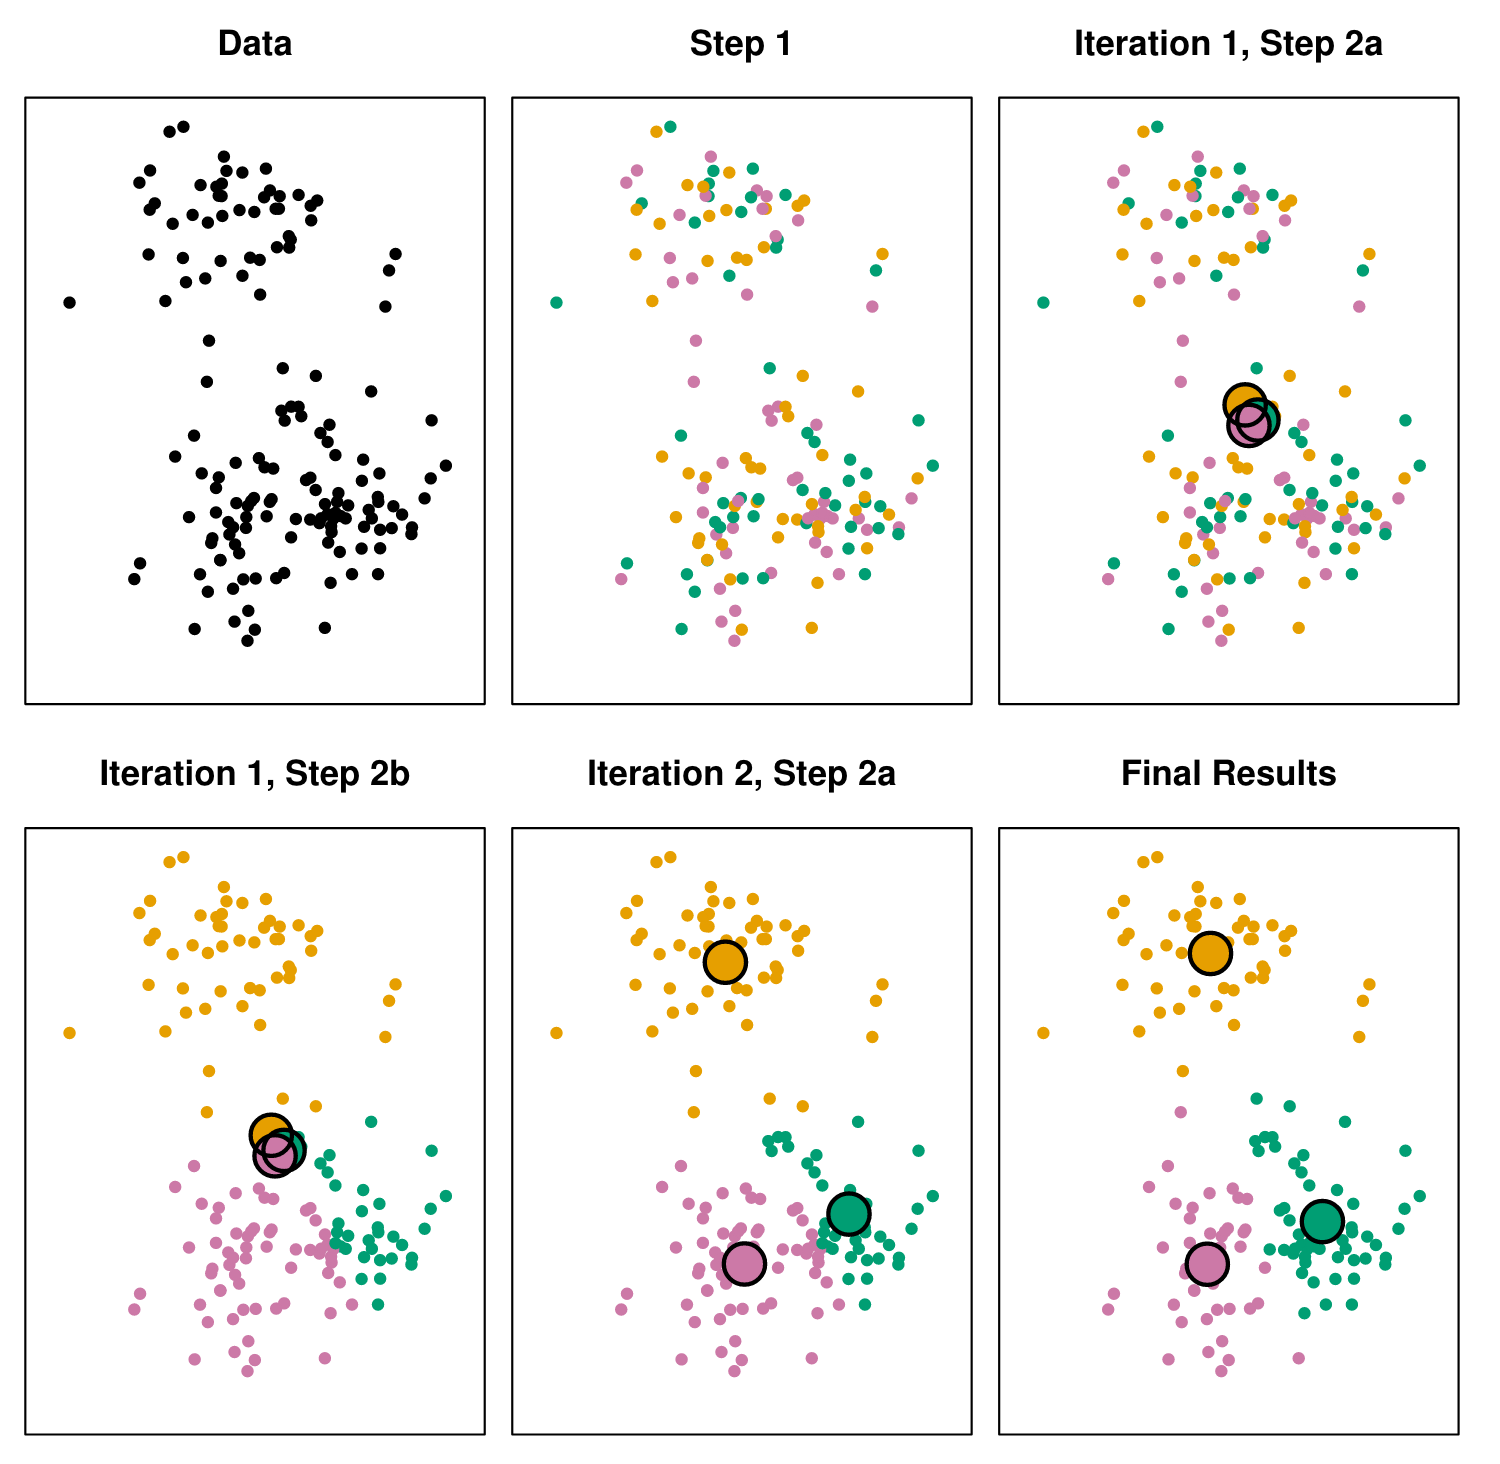
\includegraphics[width=0.6\textwidth]{Images/clustiteration.png}
    \caption[K-Means clustering iterations.]{The progress of the K-means algorithm with $K=3$ \cite{james_introduction_2021}.}
    \label{fig:clustiteration}
\end{figure}
The K-means algorithm progresses through iterative cycles involving two primary actions: (i) assigning data points to clusters and (ii) updating centroids. Given the $K$ centroids, the assignment phase allocates each data point to its nearest centroid, resulting in distinct clusters, where each cluster $C_i$ consists of points closer to its centroid $\bm{\mu}_i$ than to any other centroid. Then, in the update phase, each cluster's centroid is recalculated based on its (updated) member data points. This iterative process of assignment and updating continues until the centroids stabilize. In practical terms, K-means can be considered stable when there's no shift in centroid positions between consecutive iterations. We can adjust the tolerance parameter $\epsilon \geq 0$ for early termination of the algorithm or let the algorithm converge to the local optimum until observations no longer change cluster. In algorithm \ref{alg:kmeans}, there is the pseudo-code of the K-Means clustering algorithm.
\begin{algorithm}
\small
    \caption{K-Means Clustering}
    \label{alg:kmeans}
    \begin{algorithmic}[1]
    \STATE {$t=0$}
    \STATE {Randomly initialize $K$ centroids: $\bm{\mu}_1^t, \bm{\mu}_2^t, \dots, \bm{\mu_k^t} \in \mathbb{R}^p$}
    \REPEAT
    \STATE {$t \leftarrow t + 1$}
    \STATE {$C_i \leftarrow \empty$ for all $i=1,\dots,K$}
    \STATE {//Cluster assignment step}
    \FORALL{$\mathbf{x}_j\in D$}
    \STATE {$i^* \leftarrow \arg \min _i\left\{\left\|\mathbf{x}_j-\boldsymbol{\mu}_i^{t-1}\right\|^2\right\}$}
    \STATE {$C_{i^*} \leftarrow C_{i^*} \cup\left\{\mathbf{x}_j\right\} / / \text { Assign } \mathbf{x}_j \text { to closest centroid }$}
    \ENDFOR
    \STATE {//Centroid update Step}
    \FORALL{$i=1,\dots,K$}
    \STATE{$\boldsymbol{\mu}_i^t \leftarrow \frac{1}{\left|C_i\right|} \sum_{\mathbf{x}_j \in C_i} \mathbf{x}_j$}
    \ENDFOR
    \UNTIL{$\sum_{i=1}^k\left\|\boldsymbol{\mu}_i^t-\boldsymbol{\mu}_i^{t-1}\right\|^2 \leq \epsilon$}
    \end{algorithmic}
\end{algorithm} 
Since the initial guess of the centroids can lead to different labeling of the same observation, the K-means algorithm is typically run several times. In bagging clustering, we run the algorithm multiple times, and the final label is defined by majority voting across the different intermediate clusterizations.
% <<< End of K-means clustering algorithmclassification


% Principal component analysis >>>
\subsection{Principal Component Analysis}
\label{subsec:PCA}
Another unsupervised machine learning technique is the principal component analysis (PCA). This method leverages the information patterns within the dataset to reduce the problem's dimensionality. Principal components (PC) of a set of data in $\mathbb{R}^p$ provide a sequence of best linear approximation to that data of all ranks $q\le p$ \cite{james_introduction_2021, tibshirani_elements_2008}. \emph{Principal component analysis} refers to the process by which principal components are computed. Suppose we have a dataset that represents experience $\mathbf{E}$ of a certain phenomenon, of unlabeled data and each realization $\mathbf{x}_j \in \mathbb{R}^p$ for all $j=1,\dots,n$. Thus, $\mathbf{E} \in \mathbb{R}^{n\times p}$. The first principal component of a set of features $\mathbf{X}_1, \mathbf{X}_2, \dots, \mathbf{X}_p$ is the normalized linear combination of the features
\begin{equation}
    \label{eq:firstPC}
    Z_1=\phi_{11} \mathbf{X}_1+\phi_{21} \mathbf{X}_2+\cdots+\phi_{p1} \mathbf{X}_p
\end{equation}
By normalized, we mean that $\sum_{j=1}^p\phi_{j1}^2=1$. The elements $\phi_{11},\dots,\phi_{p1}$ are the loadings of the first principal component. But how can we find PCs? Suppose we want to find a linear model representing the $i$-th observation. We are trying to find a linear combination such as:
\begin{equation}
    \label{eq:pcaf}
    f(\lambda)=\bm{\mu}+\mathbf{V}_q\bm{\lambda}
\end{equation}
where $\bm{\mu}\in \mathbb{R}^p$ is a location vector, $\mathbf{V}_q$ is a $p\times q$ matrix with $q$ orthogonal unit vectors as columns, and $\bm{\lambda \in \mathbb{R}^q}$ is a vector of $q$ parameters. So, we can fit the model to the data by minimizing the sum of least squared errors:
\begin{equation}
    \label{eq:SSE}
    \min _{\bm{\mu},\left\{\lambda_i\right\}, \mathbf{V}_q} \sum_{j=1}^N\left\|\mathbf{x}_j-\bm{\mu}-\mathbf{V}_q \lambda_j\right\|^2
\end{equation}
We can partially optimize for $\bm{\mu}$ and the $\lambda_j$ to obtain
\begin{equation}
    \hat{\bm{\mu}} = \left(E\left(\mathbf{X}_1\right), E\left(\mathbf{X}_1\right), \dots, E\left(\mathbf{X}_p\right)\right)
\end{equation}
\begin{equation}
    \hat{\lambda}_j = \mathbf{V}_q^{T}(\mathbf{x}_j-\hat{\bm{\mu}})
\end{equation}
This leads to 
\begin{equation}
\label{eq:diocaro}
    \min _{\mathbf{V}_q} \sum_{i=1}^N\left\|\left(\mathbf{x}_j-\hat{\bm{\mu}}\right)-\mathbf{V}_q \mathbf{V}_q^T\left(\mathbf{x}_j-\hat{\bm{\mu}}\right)\right\|^2
\end{equation}
The $q \times q$ matrix $\mathbf{H}_q=\mathbf{V}_q\mathbf{V}_q^T$ is a projection matrix and maps each point $\mathbf{x}_j$ onto it's rank~-~$q$ reconstruction $\mathbf{H}_qx_j$, the orthogonal projection of $x_j$ onto the subspace spanned by the columns of $\mathbf{V}_q$. The solution can be expressed as follows. Stacked the centered observations into rows of an $N\times p$ matrix $\mathbf{E}$, we can construct the singular value decomposition
\begin{equation}
    \label{eq:SVD}
    \mathbf{E}=\mathbf{U}\bm{\Sigma}\mathbf{V}^T
\end{equation}
where $\mathbf{U}$ and $\mathbf{V}$ are unitary matrices and $\bm{\Sigma}$ is a $p \times p$ diagonal matrix, such that $\sigma_{11}\ge \sigma_{22} \ge \dots \ge \sigma_{pp}\ge 0$. This means that $\mathbf{u}_1$ and $\mathbf{v}_1$ correspond to $\sigma_{11}$ and are somehow more important with respect to $\mathbf{u}_2$ and $\mathbf{v}_2$ which are associated to $\sigma_{22}$ in explaining the information in $\mathbf{E}$ and so on and so forth. The columns of $\mathbf{U}$ are the basis vector of the new space, and the columns of $\mathbf{U}\mathbf{D}$ are the principal components. The $\sigma_{ii}$ are also called singular values and are the variance the $i$-th PC explains. Lastly, $\mathbf{v}_i=(\phi_{11} \dots \phi_{p1})$ re the loading vectors of such $i$-th PC.  For each rank $q$, the solution $\mathbf{V}_q$ to Eq. \ref{eq:diocaro}, consist of the first $q$ columns of $\mathbf{V}$. A good method to determine the number $q$ of principal components (PC) is to rely on the scree plot of explained variance. Indeed, the variance explained by each additional PC follows the law of diminishing returns. Therefore, we can decide how many PCs when we observe a significant knee in the graph.

\subsubsection{Handwritten Digits}
This example is  from \citeauthor{tibshirani_elements_2008} (2008).
PCA can be applied to images as well. For instance, take a dataset containing handwritten digits. Let's consider its application on the digit "3". Authors experimented on a set of 130 3s randomly sampled from a total of 658 total observations. Each image is a \numproduct{16 x 16} gray-scale image. We can see considerable variation in writing styles, character thickness, and orientation (Fig. \ref{fig:3s}). We can unfold images and treat each of them as vectors $\textbf{x}_j \in \mathbb{R}^{256}$, and we can use PCA on the dataset $\mathbf{E}\in\mathbb{R}^{256\times 130}$.
\begin{figure}
    \centering
    \subfloat[\label{fig:3s}]{
        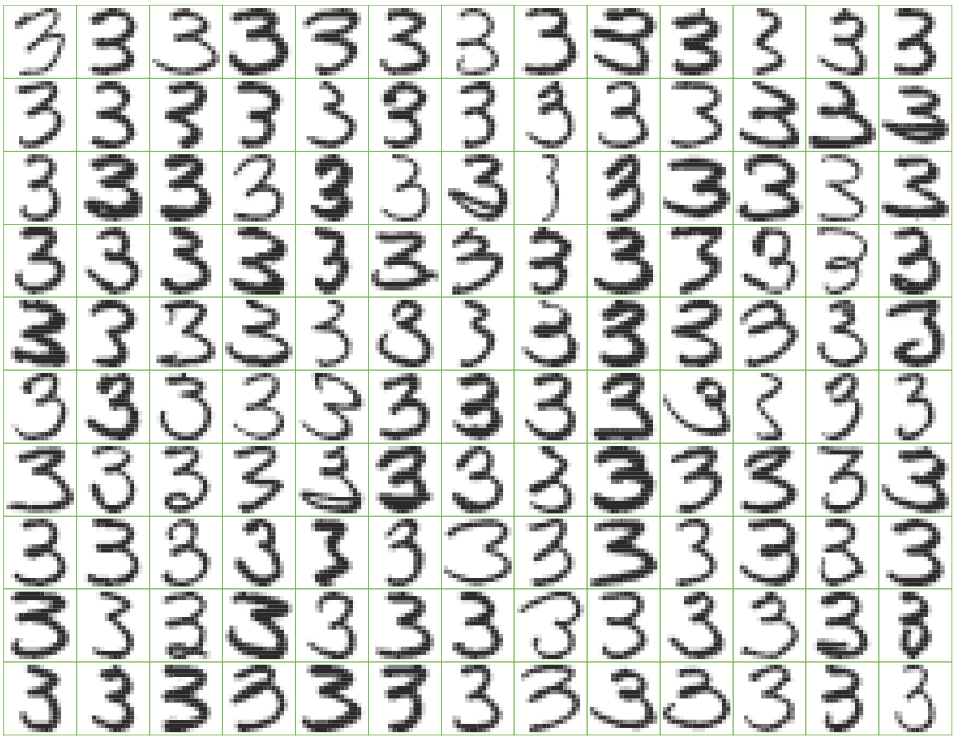
\includegraphics[scale=0.35]{Images/1303.png}
    }
    \qquad
    \subfloat[\label{fig:principal3}]{
        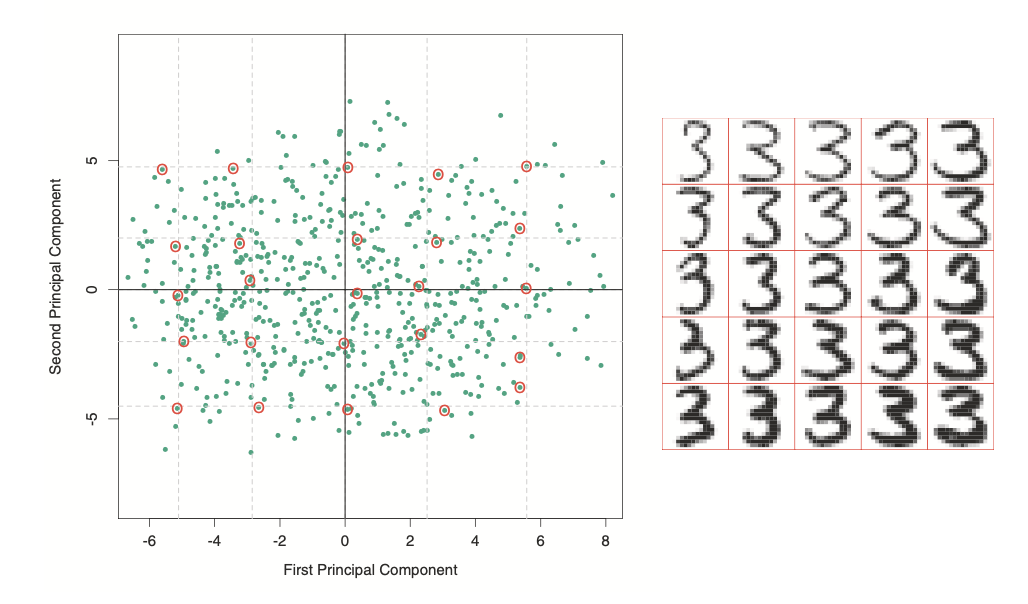
\includegraphics[scale=0.5]{Images/pc3.png}
    }
    \caption[Example of PCA of images.]{Example of PCA applaied to images dataset: the random sample of handwritten 3s (a) and the scatterplot of the first two principal components (b) with a superimposed grid in which images match red circles on the scatterplot\cite{tibshirani_elements_2008}.}
\end{figure}
From Fig. \ref{fig:principal3}, we can see that the first PC mainly accounts for the length of the lower tail of the three, while the second PC accounts for character thickness. Then, we can reshape every PC in a matrix and interpret them as images. These images will be the base for the new vectorial space. Using just 50 PCs, we can explain 90\% of the variance of all the 3s, while with 12 PCs, we can account for 63\% of the total variance.
% <<< End of Principal component analysis

%%%%%
%%%%%


% Deep Learning, ANN and CNN >>>
\subsection{Artificial Neural Network and Deep Learnig}
\label{subsec:deepl}
In 1956, there was a summer research project on artificial intelligence at Dartmouth University. A team of professors and an expert from IBM Corporation began to think about the possibility of creating virtual neural networks. These networks would learn and enhance the purpose for which they were designed through a self-improvement process, and they could be based on the mathematical model of the human brain \cite{mccarthy_proposal_1955}. Indeed, the human brain model is especially well-suited for computational purposes. The human brain possesses a massive amount of computing units: the neurons. Approximately \num{e11} neurons in an adult human brain form about 7,000 synaptic connections with other neurons, amounting to nearly \num{e15} total synapses. Moreover, the computational model of the brain is distributed among simple nonlinear units, redundant and fault-tolerant, and capable of performing calculations in parallel \cite{matteo_matteucci_perceptrons_2021}. The mathematical virtual model of a single neuron is called a perceptron, the unitary computational unit of artificial neural networks (ANN). Just like in human neurons, the perceptron has dendrites that "collect" the charge from synapses, and once a certain threshold is exceeded, the accumulated charge is released and sent to other perceptrons. The portion of the schema in Fig. \ref{fig:perceptron} enclosed in the dashed line is called the activation function and is responsible for releasing the perceptron's accumulated charge. There are various activation functions, with some of the most common ones can be seen in Fig. \ref{fig:actfunc}.
\begin{figure}
    \centering
    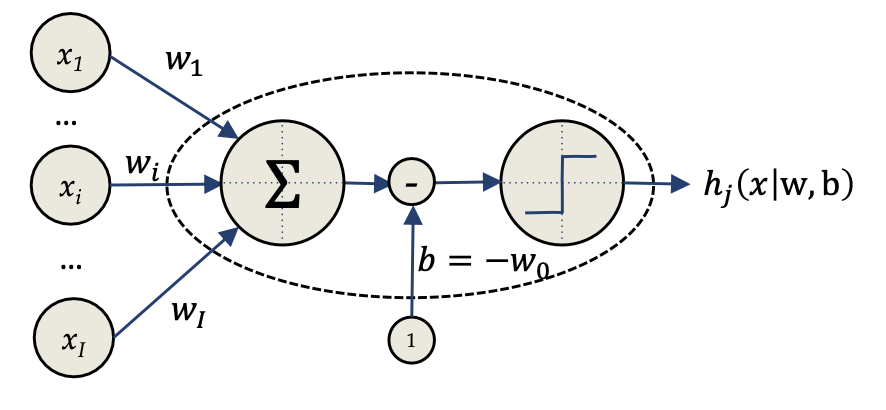
\includegraphics[width=0.6\textwidth]{Images/neurone.png}
    \caption[Perceptron schema]{Perceptron schema \cite{matteo_matteucci_perceptrons_2021}.}
    \label{fig:perceptron}
\end{figure}
Perceptrons can be combined to form networks with a layered architecture. Indeed, every neural network will have an input layer, an output layer, and a varying number of intermediate layers, known as hidden layers. Deep learning is a subfield of artificial intelligence (AI) and machine learning that involves training artificial neural networks on vast amounts of data to perform classification or regression tasks. ANNs can learn from experience $\mathbf{E}$ and understand complex patterns in data. Deep feedforward networks, also called simply feedforward neural networks or multilayer perceptrons (MLPs), are used to approximate some function $f^*$. Let's take as an example a classifier. Given an unknown function $\Lambda_0:E \rightarrow \{1,\dots,L\}$ where $\{1,\dots,L\}$ are label classes, the $f^*$ is the best approximation of the function $\Lambda_0$, defining a mapping $\mathbf{y}=f^*\left(\mathbf{x}, \bm{\theta} \right)$. The ANN learns the value of parameters $\bm{\theta}$ from $\mathbf{E}$, resulting in the best function approximation. These models are called feedforward because information flows through forward all in the network. To understand how neural networks learn from experience $\mathbf{E}$ using the chain rule and the back-propagation mechanism, readers are referred to \citeauthor{goodfellow_deep_2016} (2016).
\begin{figure}
    \centering
    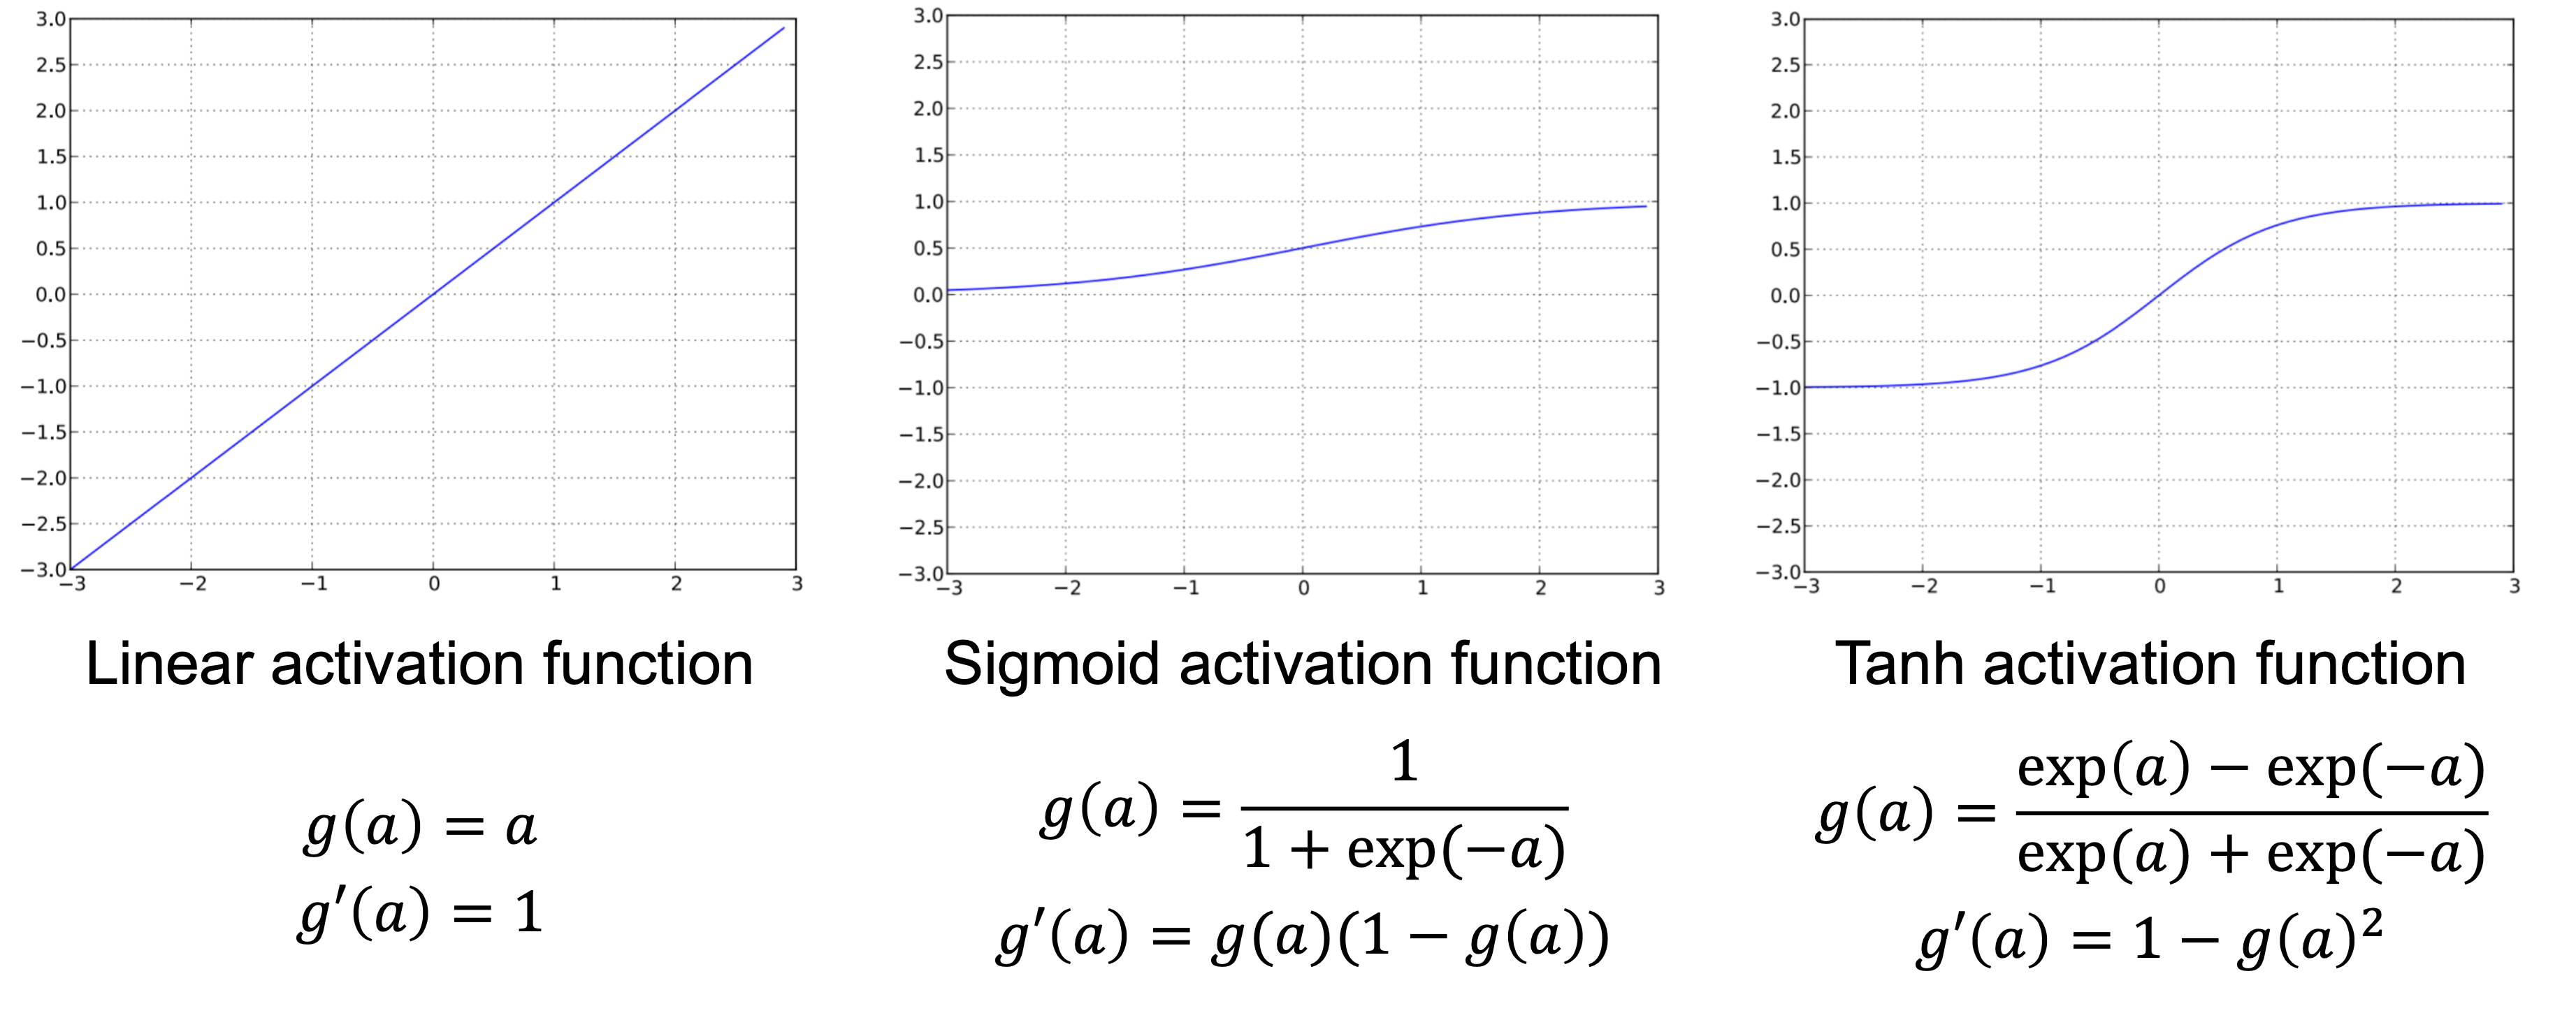
\includegraphics[width=0.8\textwidth]{Images/activationfunction.png}
    \caption[Activation functions.]{Some examples of activation functions with relatives analytical forms \cite{matteo_matteucci_perceptrons_2021}.}
    \label{fig:actfunc}
\end{figure}
Let's examine examples of how networks can address classic machine learning problems such as regression and classification. A best practice is to use tanh or sigmoid as hidden layers activation functions. Indeed, the main difference is the activation function of the output layer: 
\begin{itemize}
    \item \textbf{Regression:} since the output of a regression problem spans all $\mathbb{R}$, the activation function of the output layer will be a linear activation function;
    \item \textbf{Binary Classification:} in binary classification, the output domain is $\Omega=\{0, 1\}$. Thus, the necessary activation function for the output layer is the sigmoid activation function. The value of the function can be interpreted as class posterior probability;
    \item \textbf{Multi-class Classification:} when dealing with multiple classes ($K$), we need to use as many neurons as classes, and each output neuron will use a softmax unit. The unique feature of this activation function is that the sum of the outputs from the $K$ output neurons is equal to 1. Thus, the $k$-th output can be viewed as the probability that the input belongs to the $k$-th class.
\end{itemize}
Another typical application of neural networks is as classification algorithms for images in computer vision. However, images cannot be used directly as input since they carry too much information. We need some intermediate steps to extract useful information and reduce the problem's dimensionality by computing a feature array that summarizes the initial image's information \cite{giacomo_boracchi_convolutional_2021}. The feature array for the input layer of the classification algorithm will have a dimension of $d\ll r_1 \times c_1$ where $r_1$ and $c_1$ are the rows and the columns of the matrix representation of the image. Recall that an image can be represented as a three-dimensional matrix: the first two dimensions are pixel indexes, and the third identifies the pixel's color based on the color profile used. Take, for instance, the image in figure \ref{fig:cazzle}. The image has a width of 472 pixels a height of 376 pixels, and uses an RGB color profile. This means that three values are needed to identify the color of each pixel uniquely: the first for red, the second for green, and the third for blue. This means that we would require \numproduct{472 x 376 x 3} input neurons, one for each value of each color of each pixel of the image (more than 500,000 neurons). Feature extraction algorithms can be categorized as hand-crafted or data-driven features. With hand-crafted algorithms, we can leverage prior knowledge of the phenomenon, and features are interpretable, allowing us to exploit them even with limited data. However, this approach demands significantly more time and design/programming efforts. Moreover, it is very domain-specific and isn't so much "portable". On the other hand, data-driven feature extraction algorithms are less interpretable but offer a more robust mathematical foundation. Convolutional Neural Networks (CNNs) are neural networks that can be used for data-driven feature extraction. Given the matrix representation of the image discussed earlier, while in ANN, we talked about layers, in CNNs, we will have volumes. As the depth of such volumes increases, the height and width of the volume decreases. CNNs enable us to perform some fundamental operations essential for accurate feature extraction.
\paragraph{Convolution.} Convolutional layers "mix" all the input components. Convolution is an operation that allows us to combine all the input values from a specific region into a linear combination. Specifically, the convolution is described by the following equation:
\begin{equation}
    \label{eq:convolution}
    y_j=\sum_iw_{ij}x_i+b_j
\end{equation}
The linear combination operation is also referred to as filtering, and the parameters of this combination are called filters. The same filter is used as a sliding window through the whole spatial extent of the input images. In Fig. \ref{fig:convmatrice}, a typical convolution operation is graphically represented.
\begin{figure}
    \centering
    \subfloat[\label{fig:cazzle}]{
    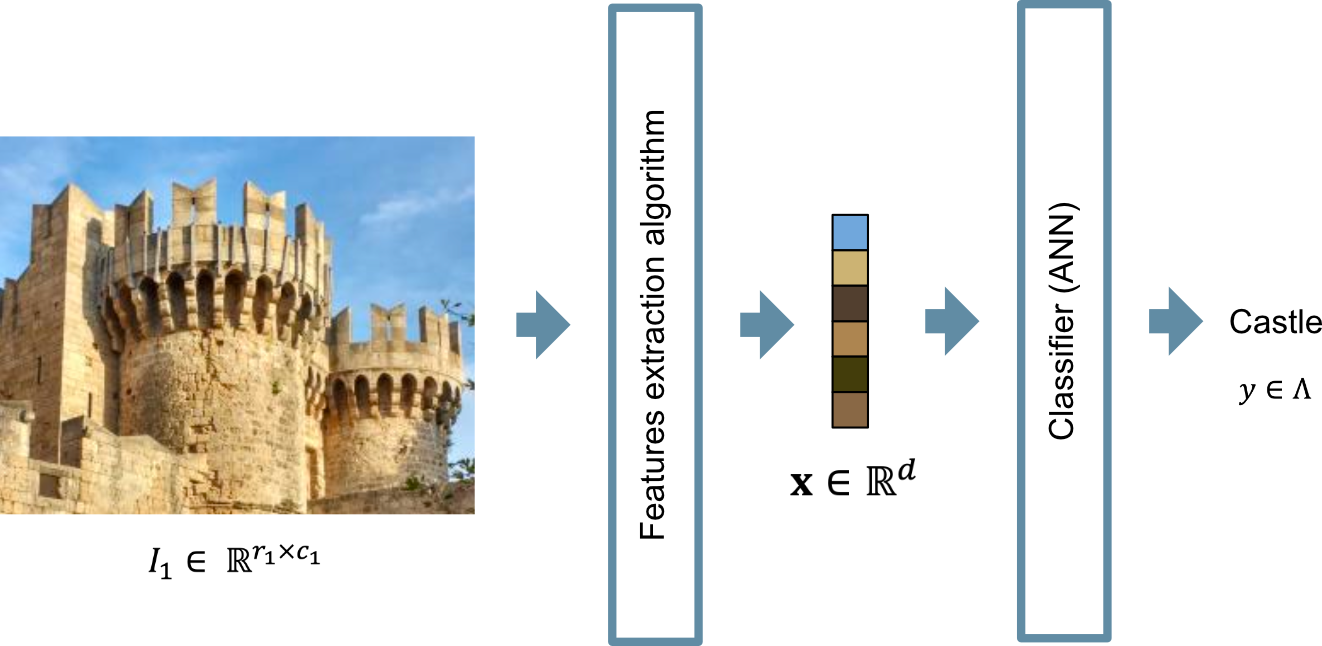
\includegraphics[width=0.7\textwidth]{Images/featureextraction.png}
    }
    \qquad
    \subfloat[\label{fig:convmatrice}]{
    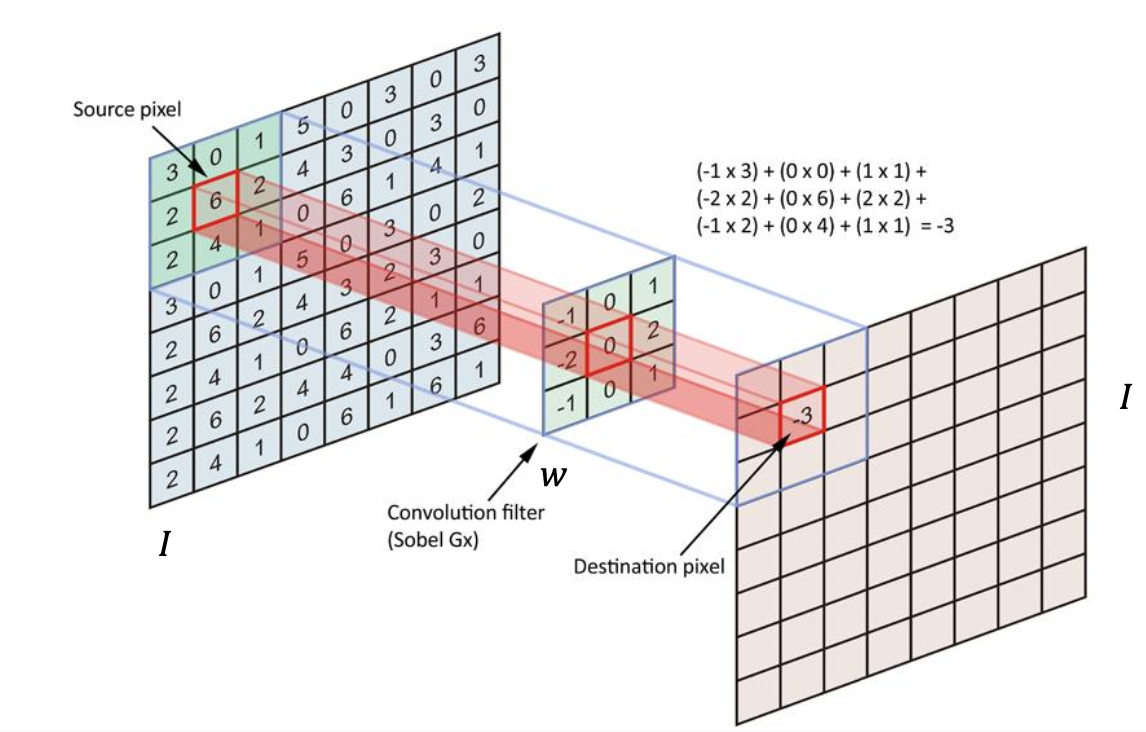
\includegraphics[width=0.5\textwidth]{Images/convolution.png}}
    \caption[Convolution operation.]{Feature extraction operation (a) adapted from \cite{giacomo_boracchi_convolutional_2021}, and convolution operation graphically represented (b)\cite{giacomo_boracchi_convolutional_2021}.}
\end{figure}
In practice, the convolution operation can be viewed as a two-dimensional window that slides across the entire image, producing an output that is a linear combination of the matrix values and their corresponding values.
\paragraph{Poolig layers.} Pooling layers reduce the spatial size of the input volume. Using the logic of a sliding window that traverses the image, a specific function is applied, often the maximum, to spatially resize the input.
\begin{figure}
    \centering
    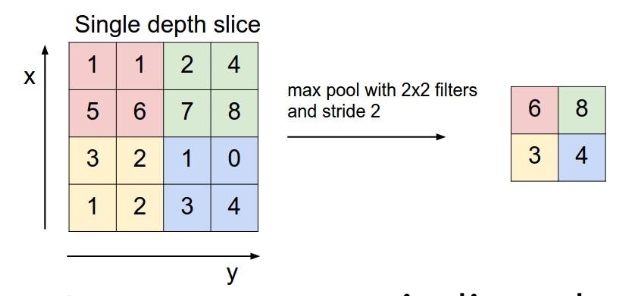
\includegraphics[width=0.5\textwidth]{Images/pooling.png}
    \caption[Pooling layer.]{Example of pooling layer that performs a max operation \cite{giacomo_boracchi_convolutional_2021}.}
    \label{fig:poolingmax}
\end{figure}
The stride parameter specifies how many elements the window shifts at once. In the figure, the window will move by two pixels simultaneously on the y-axis.
\paragraph{Activation layers.} Activation layers are used to introduce non-linearities in the network; otherwise, CNN might be equivalent to a simple linear classifier. In practice, they are layers of neurons characterized by activation functions that introduce non-linearity into the levels, just as in ANNs. We have yet to discuss two commonly used functions in these layers: the RELU (rectified linear units) and LEAKY RELU activation. The former is described as
\begin{equation}
    \label{eq:RELU}
    T(x)=\left\{\begin{array}{rr}
    x, & \text { if } x \geq 0 \\
    0, & \text { if } x<0
\end{array}\right.
\end{equation}
Whereas LEAKY RELU is similar to RELU but incorporates a slight slope for negative values, preventing neurons from dying off and becoming unresponsive after several layers. For a deeper understanding of this topic, one can refer to the vanishing gradient problem as discussed by Goodfellow.
\begin{equation}
    \label{eq:LEAKYRELU}
    T(x)=\left\{\begin{array}{rr}
    x, & \text { if } x \geq 0 \\
    k\cdot x, & \text { if } x<0
\end{array}\right.
\end{equation}
where $k$ is usually in the order of $10^{-2}$.
The convolution output will be a dense feature layer, which implies that this layer can serve as input for an ANN, which will have as many output neurons as classes in the original domain. Fig. \ref{fig:typicalcnn} shows an example of how a general CNN works.
\begin{figure}
    \centering
    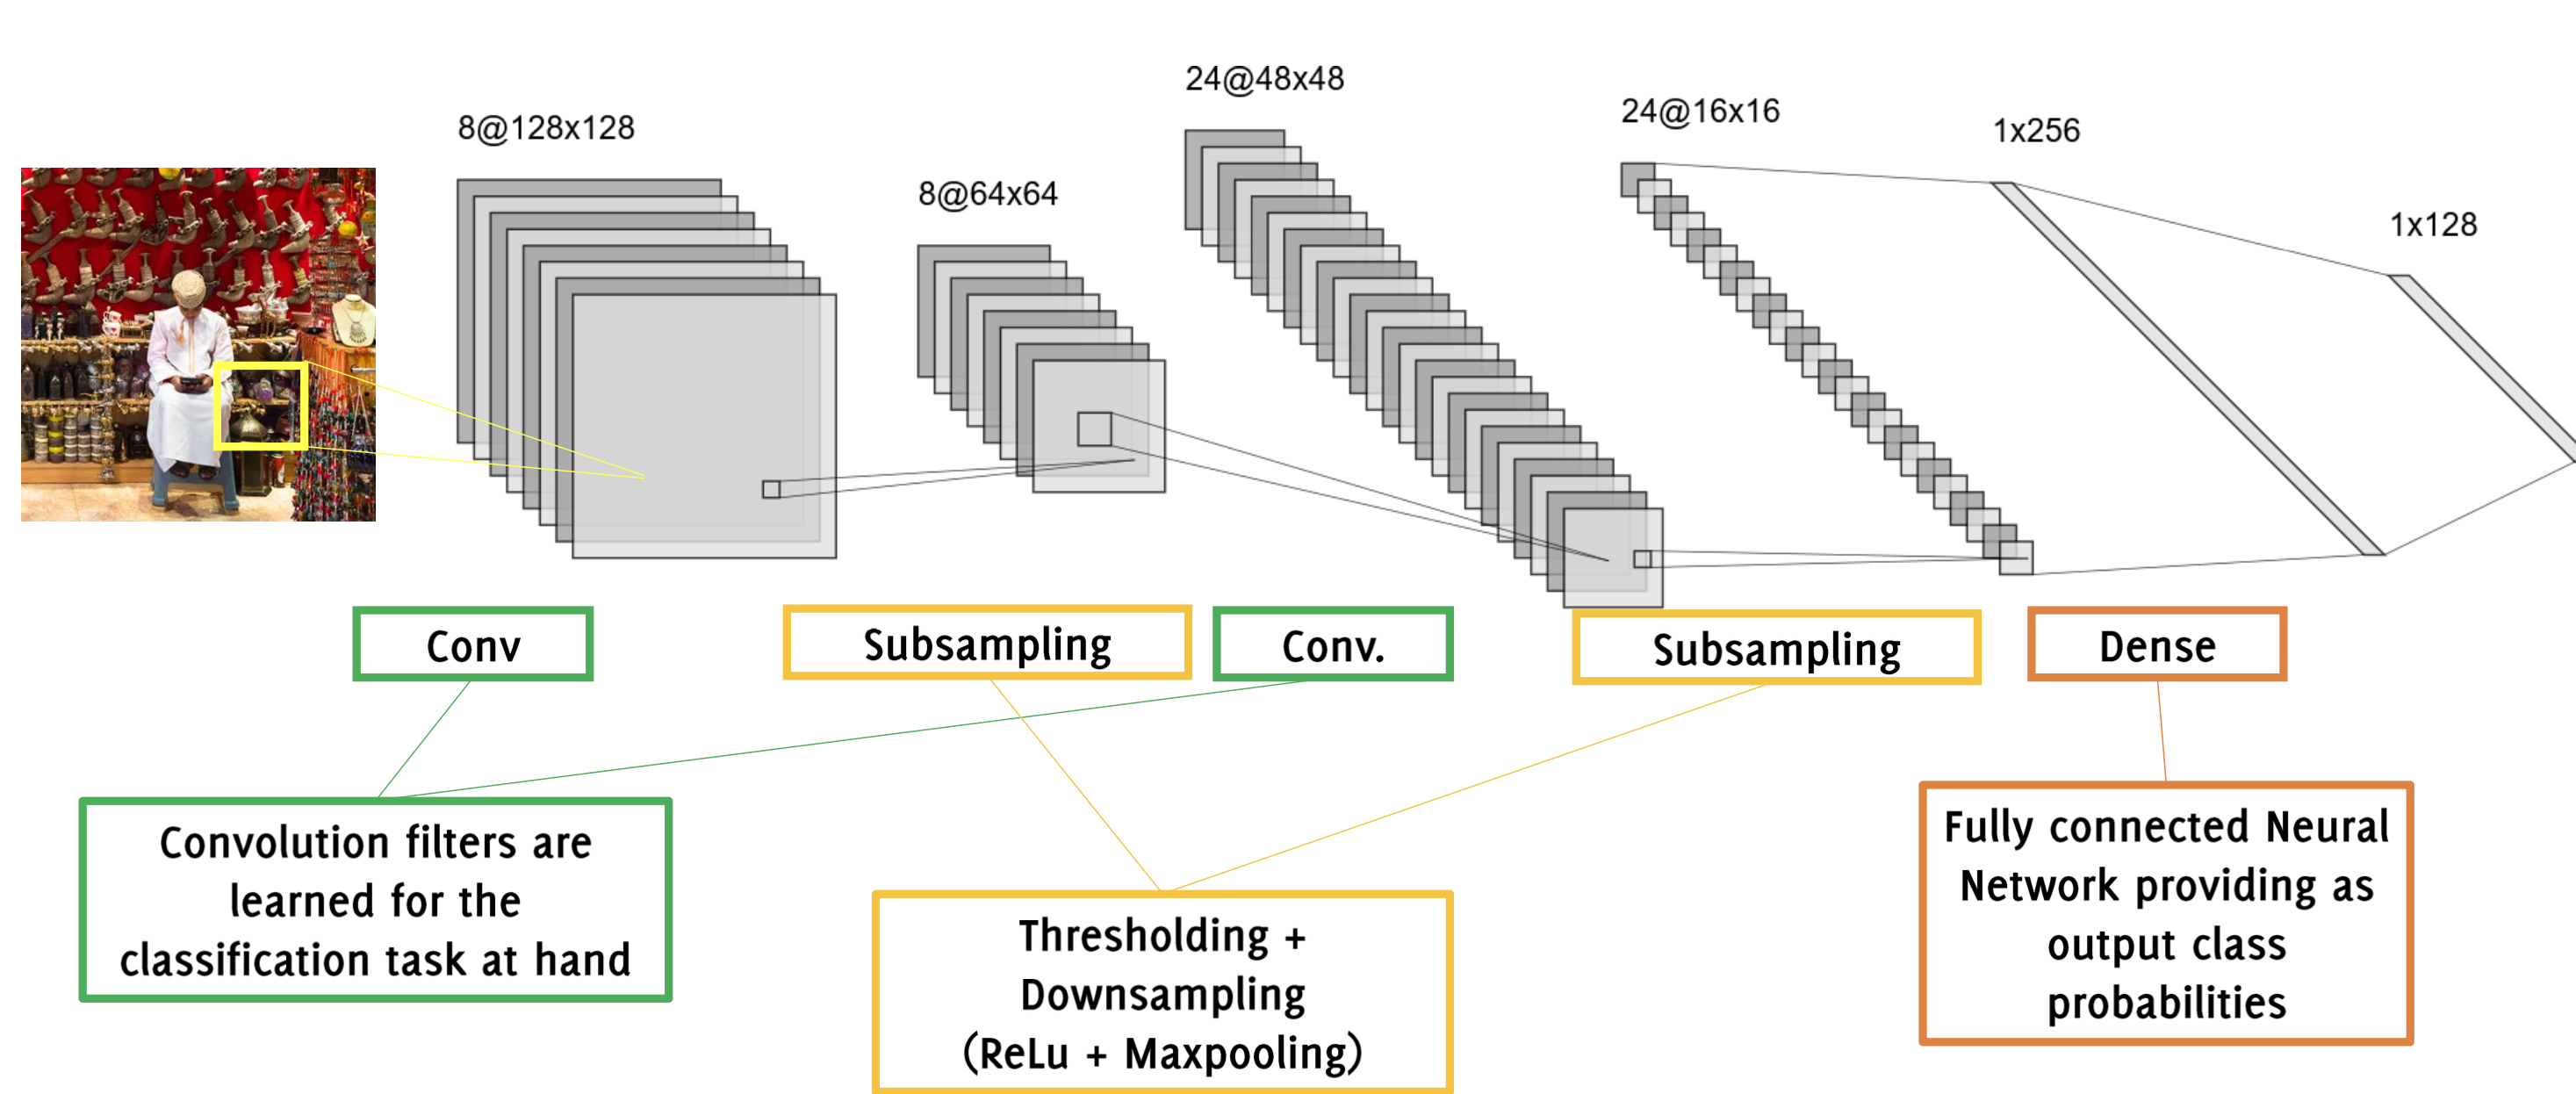
\includegraphics[width=0.8\textwidth]{Images/CNNtypical.png}
    \caption[CNN general structure.]{Graphical representation of a tipical CNN used for image classification \cite{giacomo_boracchi_convolutional_2021}.}
    \label{fig:typicalcnn}
\end{figure}
% End of Deep learning, ANN and CNN

%%%%%
%%%%%

% Hot spot >>>
\section{Hot-Spot Detection Using ML Algorithm: A-State-Of-The-Art Review}
\label{sec:hotspotstateart}
% <<< End of Hot spot 